\chapter*{Conclusion --- \textit{The Rosetta Stone}}
\addcontentsline{toc}{chapter}{Conclusion}
\markboth{Conclusion}{Conclusion}
\label{conclusion}



\bigskip


\section{The Rope-Stretcher's Return}

Let us go back to the Nile.

Our rope-stretcher --- the \textit{harpedonaptai}, as the Greeks called him --- is older now. His hands are calloused, his rope frayed at the knots. He has spent his career planting stakes and pulling cord into $3$-$4$-$5$ triangles, and he has never once questioned why the trick works. But his apprentice, who has been reading this book over the pharaoh's shoulder, pulls him aside one evening and says:

"Master, do you know what your triangle \textit{is}?"

The surveyor shrugs. "It is a right angle. It squares the field."

"It is much more than that," the apprentice says. And she begins to list the identities of this humble shape --- the secret lives of the $3$-$4$-$5$ triple --- and as she speaks, the surveyor's world cracks open like an egg, revealing a universe inside.

\begin{figure}[htbp]
\centering
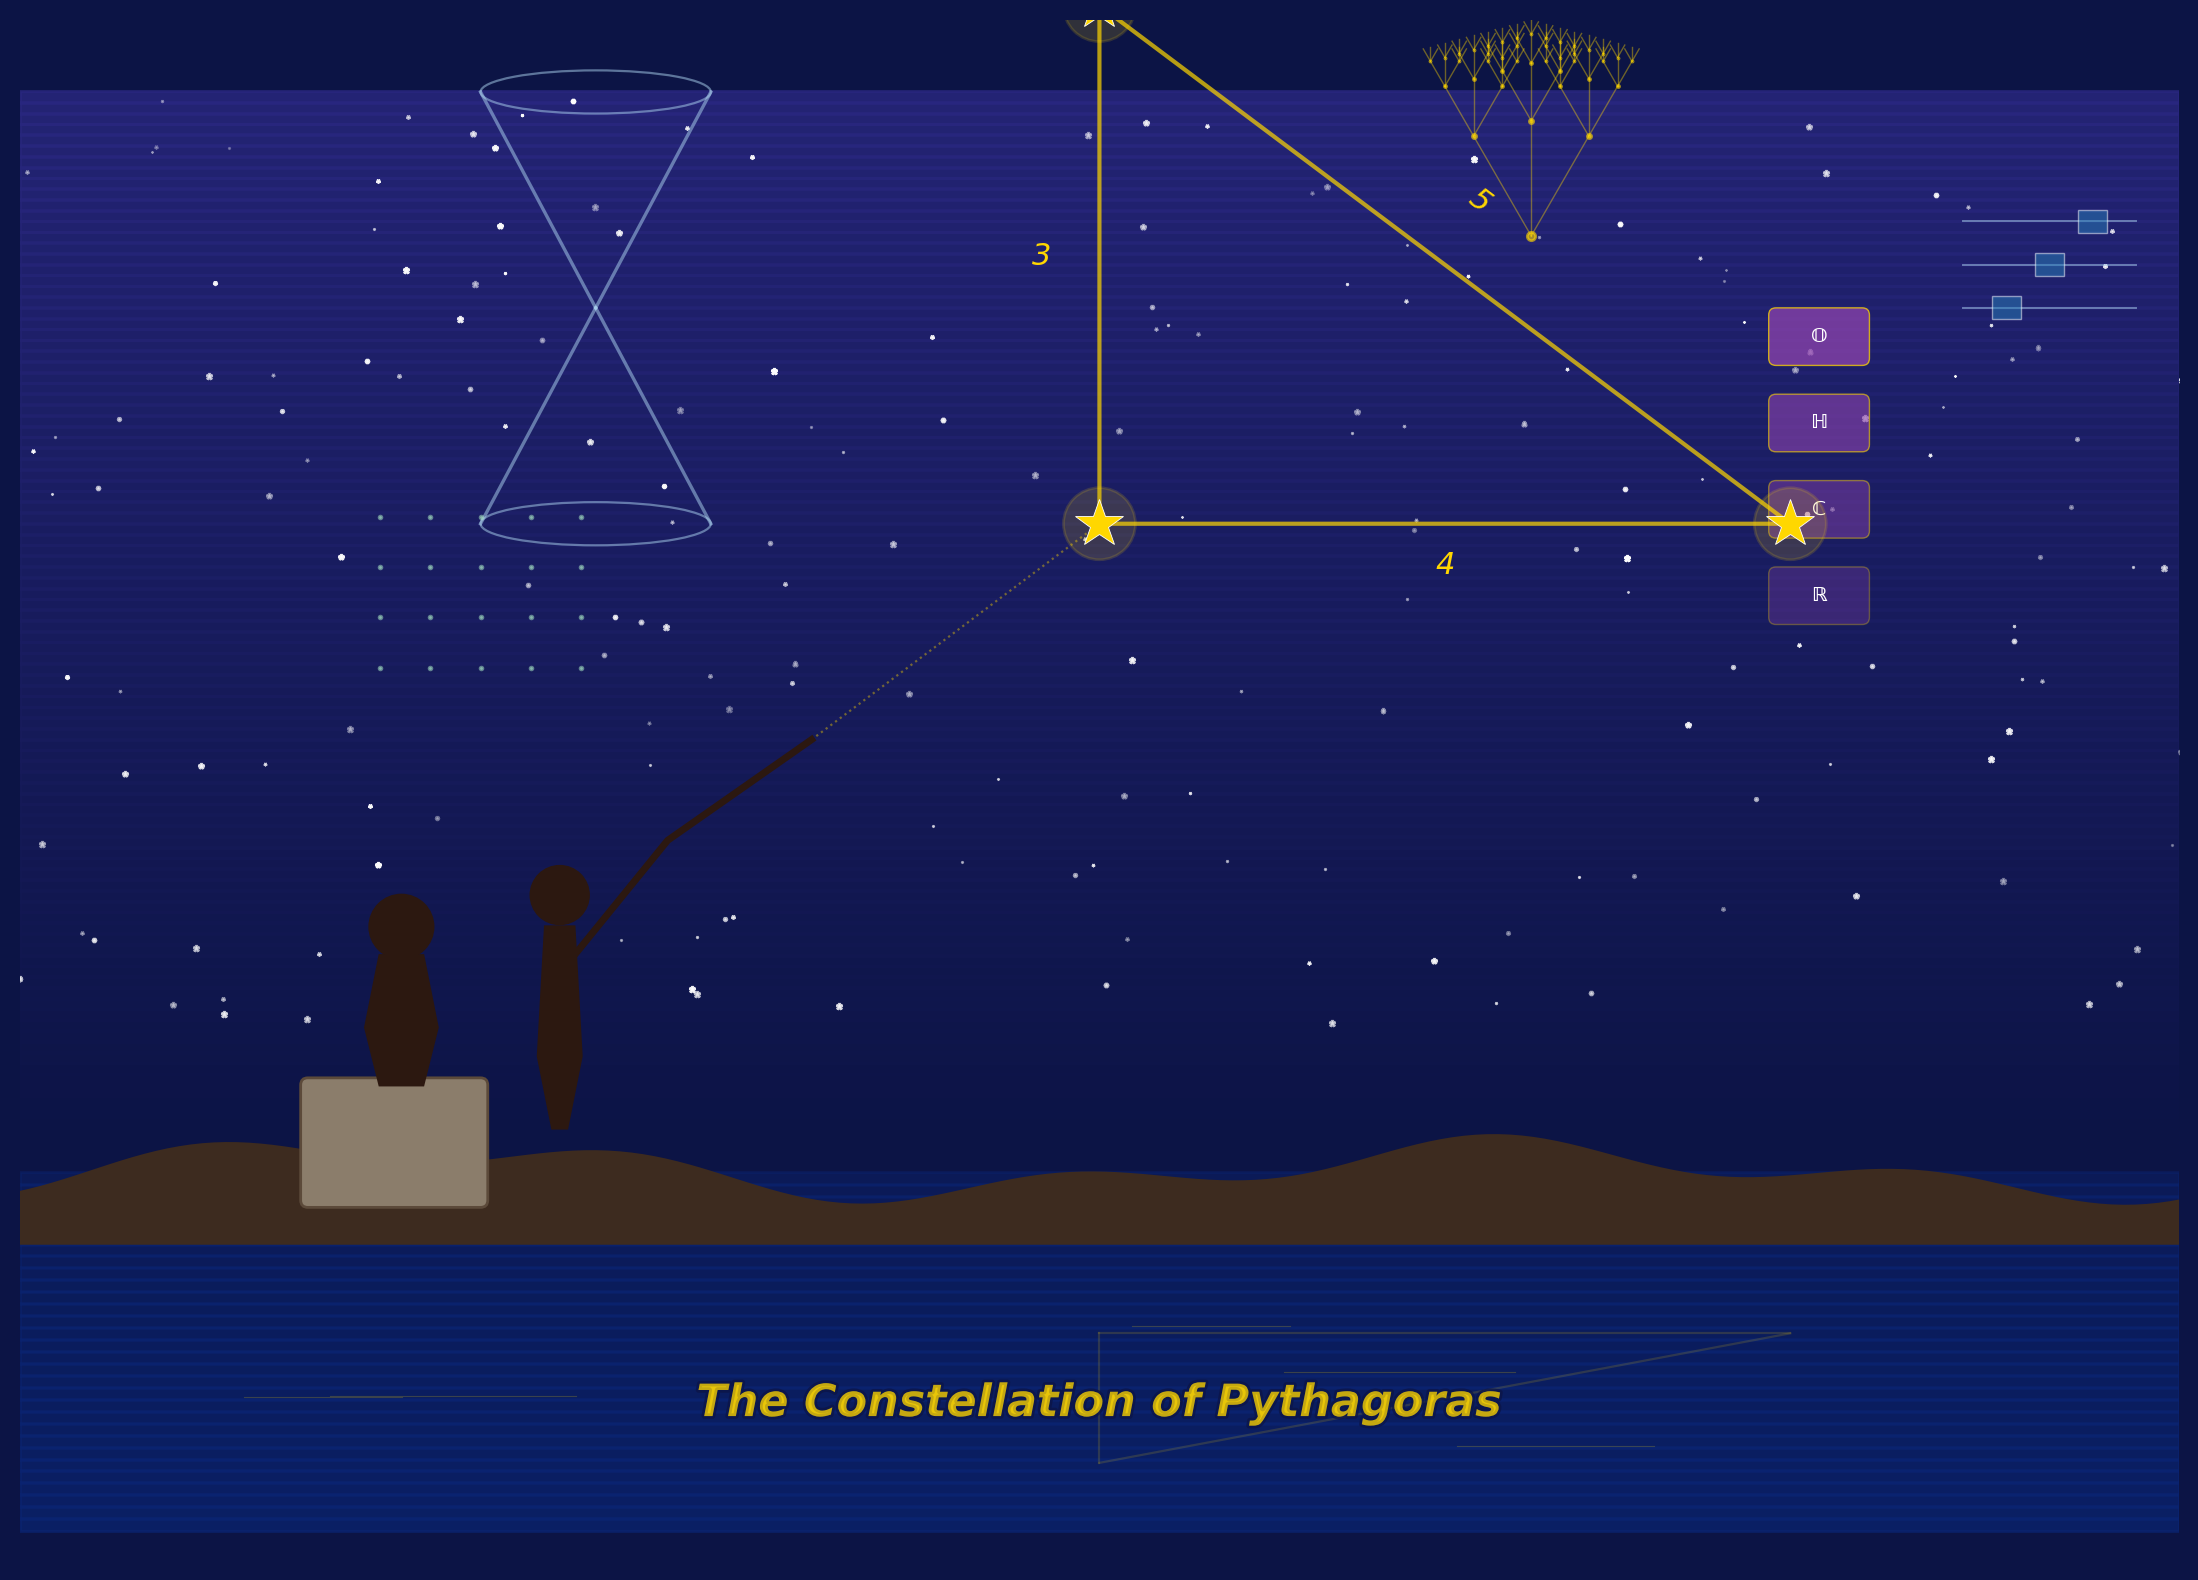
\includegraphics[width=0.82\textwidth]{../Conclusion/images/fig01_rope_stretcher_return.png}
\caption{An aged Egyptian rope-stretcher sits on a limestone block beside the Nile at dusk. His apprentice stands beside him, gesturing at the sky, where the stars have rearranged themselves into a web of\ldots}
\end{figure}


\bigskip


\section{Nine Faces of One Equation}

Here, then, is what the apprentice knows --- and what you, reader, now know with her.

\textbf{Face 1: The Seed of an Infinite Tree.} The triple $(3, 4, 5)$ is not one of many isolated curiosities. It is the \textit{root} of a ternary tree --- the Berggren tree --- in which every primitive Pythagorean triple appears exactly once. Three matrices, $\mathbf{A}$, $\mathbf{B}$, and $\mathbf{C}$, act as begetting operations, and the equation
\index{Pythagorean triple}
\index{Pythagorean triple!primitive}
\index{Berggren tree}
\index{Berggren, B.}
\index{matrix}

\[
\mathbf{B}^{\!\top} \mathbf{Q}\, \mathbf{B} = \mathbf{Q}, \qquad \mathbf{Q} = \operatorname{diag}(1, 1, -1),
\]

guarantees that every child is again Pythagorean. The tree is not an accident. It is the orbit of a single point under a discrete group of symmetries --- a \textit{group-theoretic skeleton} supporting an infinite family of triangles. We grew this tree in the opening chapter, and every branch we explored thereafter led somewhere astonishing.

\textbf{Face 2: A Point on Einstein's Light Cone.} The quadratic form $Q(a, b, c) = a^2 + b^2 - c^2$ is the Minkowski metric of $(2{+}1)$-dimensional spacetime. Our Pythagorean triples live on the null cone $Q = 0$ --- the same surface that light rays trace through the cosmos. The Berggren matrices generate a discrete subgroup of the Lorentz group $O(2,1;\mathbb{Z})$, and the formula for inverting them,
\index{Berggren matrices}
\index{quadratic form}
\index{Lorentz group}
\index{null cone}
\index{light cone}
\index{Minkowski space}
\index{spacetime}

\[
\mathbf{B}^{-1} = \mathbf{Q} \cdot \mathbf{B}^{\!\top} \cdot \mathbf{Q},
\]

is precisely the formula relativists use to invert Lorentz boosts. Minkowski's geometry, born to describe continuous spacetime, secretly organizes the most ancient discrete objects in number theory. The irony is exquisite: the pharaoh's surveyor was doing special relativity with a rope.

\textbf{Face 3: The Euclidean Algorithm in Disguise.} Climbing \textit{down} the Berggren tree --- from child to parent --- turns out to be the Euclidean algorithm applied to the parameter ratio $m/n$ of the classical Pythagorean parametrization. The $2 \times 2$ inverse matrices compute continued-fraction quotients; the descent terminates at the root $(3, 4, 5)$ in exactly as many steps as $\gcd(m, n)$ takes to reach $1$. The most ancient algorithm in mathematics --- Euclid's recipe for finding greatest common divisors, circa 300 BCE --- was hiding inside a tree discovered in 1934.
\index{greatest common divisor}

\textbf{Face 4: A Lattice Vector.} Each Pythagorean triple is a point in the integer lattice $\mathbb{Z}^3$, and its Berggren ancestors trace a path through lattice basis reduction. In two dimensions, Gauss showed this reduction is already optimal: no shortcut can beat the zigzag descent, and the complexity is $\Theta(\sqrt{N})$ for a balanced semiprime $N$. This is not a failure of the method --- it is a \textit{theorem} about the geometry of planar lattices. But in three and more dimensions, the walls of optimality crack open. The LLL algorithm exploits extra dimensions to find short vectors that the planar projection misses entirely, and this is where the higher-dimensional Pythagorean objects --- quadruples, quintuplets, octuplets --- begin to earn their keep.
\index{semiprime}
\index{lattice}

\textbf{Face 5: A Factoring Machine.} Perhaps the most surprising identity of all. Given any odd composite $N$, embed it as the leg of a Pythagorean triple:
\index{factoring}

\[
N^2 + \left(\frac{N^2 - 1}{2}\right)^{\!2} = \left(\frac{N^2 + 1}{2}\right)^{\!2}.
\]

Now descend the tree. At each node, compute $\gcd(\text{leg}, N)$. If a nontrivial divisor appears --- and it \textit{must}, since the hypotenuse strictly decreases and cannot reach zero without passing through a node where the leg shares a factor with $N$ --- the composite is cracked. The difference-of-squares identity
\index{difference of squares}

\[
(c - b)(c + b) = a^2
\]

is the skeleton key, and the three roads to the safe --- Euler's two-representation method, Gaussian integer factorization, and tree descent --- all converge on the same $\gcd$.
\index{Gaussian integers}
\index{Euler, Leonhard}

\textbf{Face 6: A Rung on the Cayley-Dickson Ladder.} The Brahmagupta-Fibonacci identity,
\index{Cayley--Dickson construction}
\index{Brahmagupta--Fibonacci identity}
\index{Brahmagupta}
\index{Fibonacci}

\[
(a^2 + b^2)(c^2 + d^2) = (ac - bd)^2 + (ad + bc)^2,
\]

is the norm multiplicativity of the Gaussian integers $\mathbb{Z}[i]$. It extends to Euler's four-square identity via the quaternions $\mathbb{H}$, and to Degen's eight-square identity via the octonions $\mathbb{O}$. Each step up the ladder doubles the dimension and loses a structural property --- commutativity, then associativity, then the division property --- but each step also \textit{doubles the number of factoring channels}. A Pythagorean octuplet yields twenty-eight independent chances to find $\gcd(\cdot, N) \notin \{1, N\}$. Hurwitz's theorem tells us this ladder has exactly four rungs --- $1, 2, 4, 8$ --- and no more. The channel hierarchy is not a human choice; it is a law of algebra.
\index{quaternions}
\index{octonions}
\index{norm!multiplicativity}

\[
\mathbb{R} \xrightarrow{\text{lose order}} \mathbb{C} \xrightarrow{\text{lose commutativity}} \mathbb{H} \xrightarrow{\text{lose associativity}} \mathbb{O} \xrightarrow{\text{lose division}} \mathbb{S}
\]

\textbf{Face 7: A Quantum Search Problem.} The tree descent is deterministic --- at each node, at most one inverse branch produces a valid child --- so quantum parallelism cannot explore multiple branches simultaneously. But Grover's algorithm \textit{can} compress the sequential depth search from $O(d^*)$ to $O(\sqrt{d^*})$, yielding
\index{Grover!algorithm}

\[
O(\sqrt{d^*}) = O(N^{1/4})
\]

for balanced semiprimes. This is a genuine quadratic speedup, and it is \textit{tight}: Bennett, Bernstein, Brassard, and Vazirani proved in 1997 that Grover's bound cannot be improved. The Berggren tree reveals exactly \textit{where} quantum mechanics helps (sequential search) and \textit{where} it cannot (deterministic branching).

\textbf{Face 8: A Tropical Polynomial Root.} In the min-plus semiring --- where $a \oplus b = \min(a,b)$ and $a \odot b = a + b$ --- polynomial "roots" are determined by Newton polygon slopes rather than algebraic vanishing. This strange arithmetic provides alternative machinery for shortest-vector problems in lattices, and it marks one of many unexplored boundaries of the Pythagorean framework. The connection is speculative, tantalizing, and entirely open.
\index{semiring}

\textbf{Face 9: The Only Exponent That Works.} Fermat's Last Theorem tells us that $a^n + b^n = c^n$ has no positive integer solutions for $n \geq 3$. The Pythagorean world --- $n = 2$ --- is the \textit{unique} exponent where integer solutions are not merely possible but infinitely abundant, richly structured, and computationally useful. Fermat himself proved the $n = 4$ case using infinite descent --- the \textit{same} descent principle that drives Berggren tree factoring. The Pythagorean equation sits at the exact boundary where descent works. Beyond it lies Fermat's empty sea, and the full proof required Wiles, Taylor, and the deepest machinery of twentieth-century mathematics.
\index{Fermat!last theorem}
\index{Fermat, Pierre de}
\index{Wiles, Andrew}
\index{descent!infinite}

\begin{figure}[htbp]
\centering
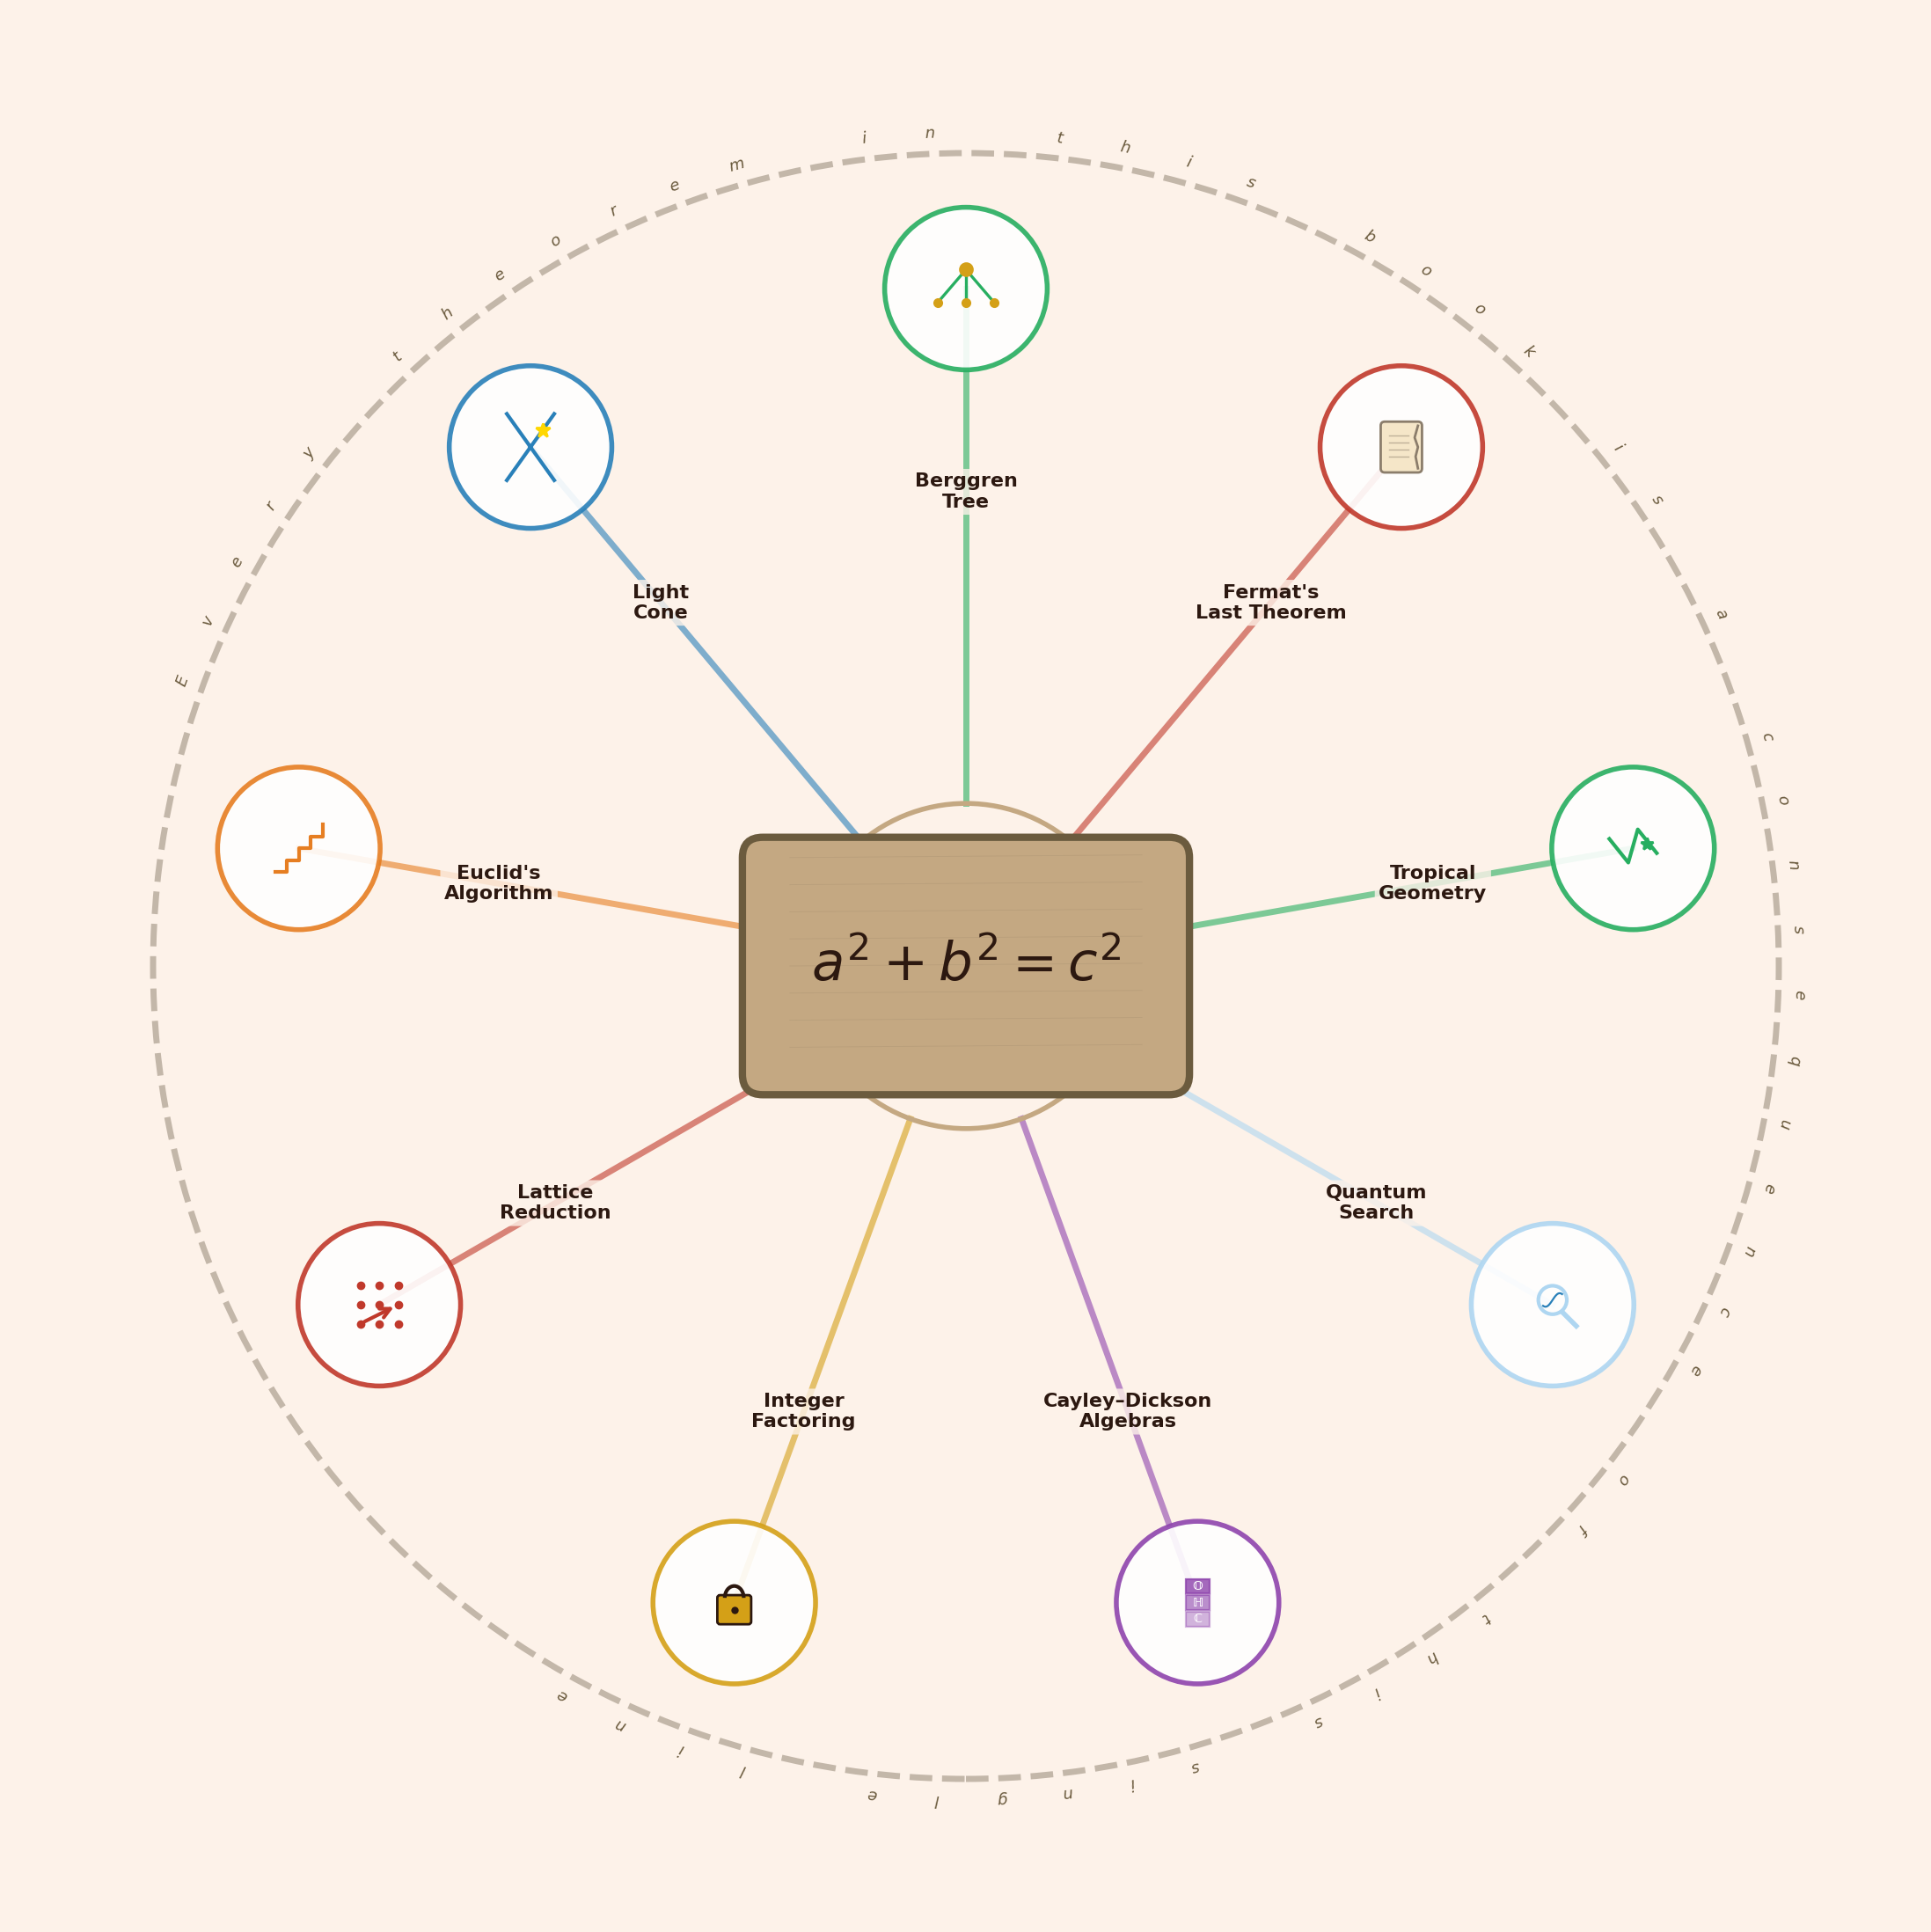
\includegraphics[width=0.82\textwidth]{../Conclusion/images/fig02_rosetta_mandala.png}
\caption{A full-page "Rosetta Stone" mandala. At the center, carved into an ancient stone tablet, is the equation $a^2 + b^2 = c^2$. Nine spokes radiate outward, each ending in an iconic vignette: (1) a\ldots}
\end{figure}


\bigskip


\section{The Unreasonable Effectiveness of a Schoolchild's Equation}

There is a phrase, due to Eugene Wigner, that haunts the philosophy of mathematics: \textit{the unreasonable effectiveness of mathematics in the natural sciences}. Wigner marveled that equations devised for pure intellectual pleasure --- group theory, non-Euclidean geometry, abstract algebra --- kept turning up as the precise language of physics. The Pythagorean equation is the oldest and most dramatic example of this phenomenon, but with a twist: its effectiveness is \textit{internal}. It is not that $a^2 + b^2 = c^2$ describes the physical world (although, via the Minkowski metric, it does). It is that this single equation, the first theorem any schoolchild learns, contains within itself the seeds of a staggering range of mathematical structures.

The Berggren tree is a group orbit. The Lorentz connection is a signature change. The lattice correspondence is a change of coordinates. The factoring algorithms are GCD computations on null-cone projections. The Cayley-Dickson hierarchy is a norm tower. The quantum bounds are information-theoretic. The tropical connection is a semiring substitution. And Fermat's Last Theorem is the statement that \textit{none of this works for any other exponent}.

Each of these observations, taken alone, would make a fine journal paper. Taken together, they form something rarer: a \textit{coherent worldview}, a way of seeing mathematics not as a collection of disconnected specialties but as a single landscape in which geometry, algebra, number theory, physics, and computation are merely different elevations of the same terrain. The Pythagorean equation is the Rosetta Stone that lets us translate between them.


\bigskip


\section{The Puzzles That Remain}

At the end of every column Martin Gardner ever wrote, there was a sense that the playground had merely been glimpsed --- that behind every solved puzzle lay three unsolved ones. This book is no different.

We do not know the structure of the Pythagorean quadruple forest. We do not know whether modular forms can predict which sum-of-squares representations yield nontrivial GCDs. We do not know whether tropical geometry can crack lattice problems. We do not know whether quantum walks on the Berggren tree, exploiting its Lorentz symmetries, can beat the $N^{1/4}$ Grover bound. And we do not know whether the octuplet channel --- twenty-eight independent factoring shots from a single representation --- is the theoretical ceiling, or whether non-associative structures beyond the octonions can still surprise us.
\index{tropical geometry}
\index{Pythagorean quadruple}

What we \textit{do} know is the complexity landscape, and it is worth stating plainly:

\[
\begin{array}{lcc}
\textbf{Method} & \textbf{Classical} & \textbf{Quantum} \\[4pt]
\hline
\\[-6pt]
\text{Trial division} & O(\sqrt{N}) & O(N^{1/4}) \\[2pt]
\text{Berggren tree descent} & \Theta(\sqrt{N}) & O(N^{1/4}) \\[2pt]
\text{Quadratic sieve} & e^{O(\sqrt{\log N \cdot \log\log N})} & ? \\[2pt]
\text{Number field sieve} & e^{O((\log N)^{1/3}(\log\log N)^{2/3})} & ? \\[2pt]
\text{Shor's algorithm} & --- & O((\log N)^3) \\[2pt]
\index{Shor!algorithm}
\end{array}
\]

The Pythagorean framework sits at the $\sqrt{N}$ boundary --- too slow for breaking modern cryptographic keys, but rich enough to illuminate the \textit{structure} of factoring in ways that sub-exponential methods, which rely on smoothness heuristics rather than geometric insight, do not. The question is whether the higher-dimensional extensions --- the quadruple forests, the octuplet channels, the lattice lifts --- can cross the barrier into sub-exponential territory. The answer is unknown. The question is magnificent.


\bigskip


\section{A Last Puzzle}

I will leave you, as Gardner always did, with a puzzle to carry away.

Consider the number $N = 1{,}000{,}003$. It is a prime. (You may verify this, though it will take some effort.) Now form its trivial Pythagorean triple:

\[
1{,}000{,}003^2 + \left(\frac{1{,}000{,}003^2 - 1}{2}\right)^{\!2} = \left(\frac{1{,}000{,}003^2 + 1}{2}\right)^{\!2}
\]

This triple sits somewhere in the Berggren tree. Its depth, by the formula we derived, is

\[
\text{depth} = \frac{1{,}000{,}003 - 3}{2} = 500{,}000.
\]

Half a million steps from the root. And yet, using repeated squaring, you can navigate to this node in roughly $\lceil \log_2 500{,}000 \rceil = 19$ matrix multiplications.

Here is the puzzle: \textit{along the way, how many other primes does your path visit?} That is --- how many intermediate triples $(a, b, c)$ encountered during the descent have a leg $a$ or $b$ that is itself prime?

I don't know the answer. Neither, as far as I can tell, does anyone. The distribution of primes along Berggren tree paths is a question that touches the deepest open problems in analytic number theory --- the Hardy-Littlewood conjectures, the distribution of primes in quadratic sequences, the Sato-Tate conjecture for modular forms. The $3$-$4$-$5$ triangle, that tired old workhorse of grade-school geometry, is \textit{still} asking questions that no one can answer.

And that, I think, is the deepest lesson of this book. Mathematics is not a finished building to be toured but an endless construction site, and the most productive hard hats are often found not at the fashionable frontiers but at the ancient foundations, where a patient eye can still spot cracks that open into caverns.

The rope-stretcher's triangle has more to tell us. It always has.

\begin{figure}[htbp]
\centering
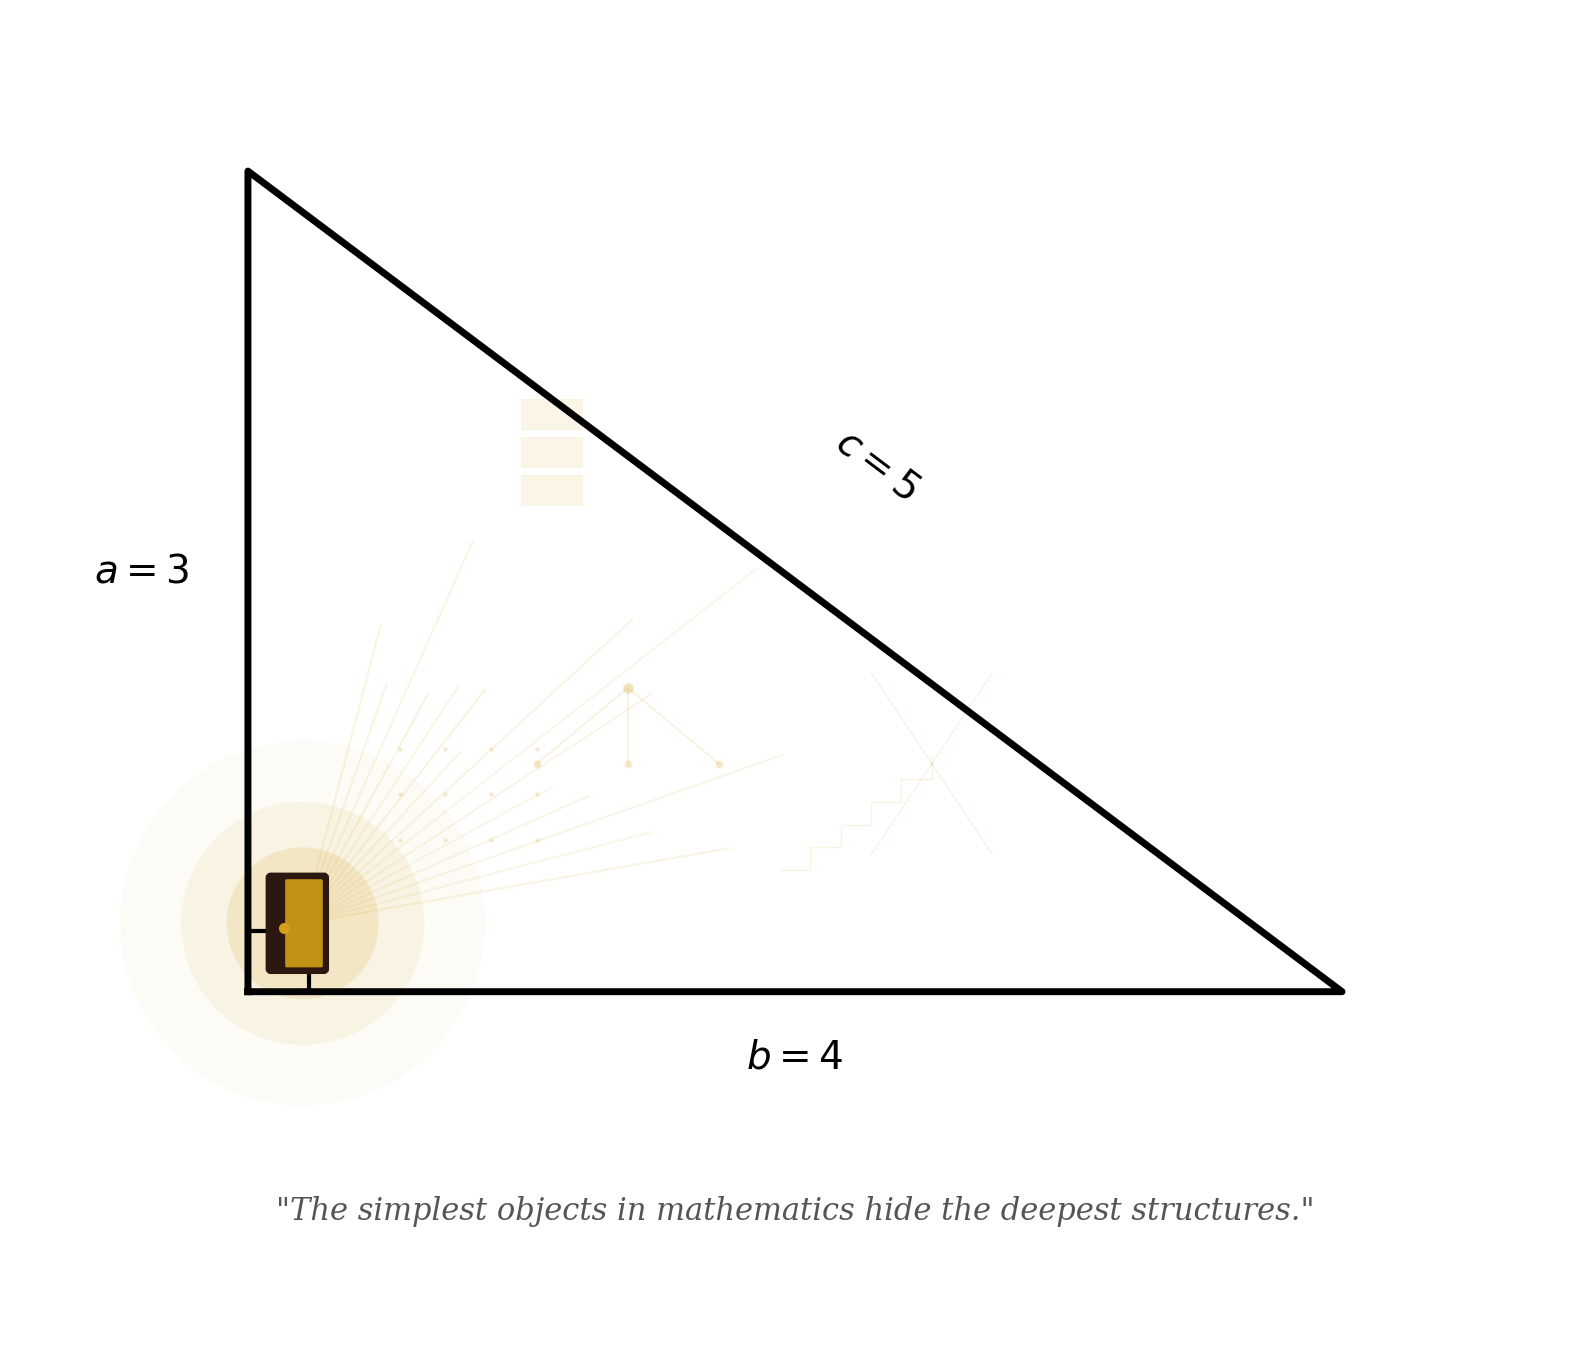
\includegraphics[width=0.82\textwidth]{../Conclusion/images/fig03_final_triangle.png}
\caption{The final image. A single $3$-$4$-$5$ right triangle, drawn in clean black ink on an otherwise empty white page. At the right-angle vertex, a tiny door stands ajar, and through it spills warm golden\ldots}
\end{figure}


\bigskip


\[
\boxed{a^2 + b^2 = c^2}
\]


\bigskip


\textit{--- Finis ---}

